\documentclass[a4paper]{article}
\usepackage{graphicx}
\usepackage{amsmath,amssymb,amstext}


\begin{document}

\subsubsection{CompareChildrenSimilar}

  \begin{description}
  
  \item[testcase\_01:] 2 Gleiche Modelle. 100\% �bereinstimmung.
    
   \begin{equation*}
   Similarity = \frac{1+1+1}{3}=1
   \end{equation*}

  
    
	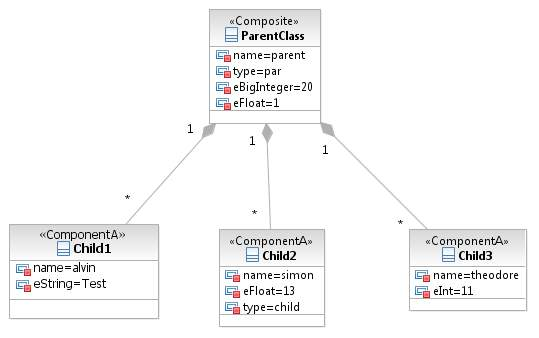
\includegraphics[scale=0.5]{CompareChildrenMatchedOrSimilarTestScreens/Testcase01model1.jpeg}
	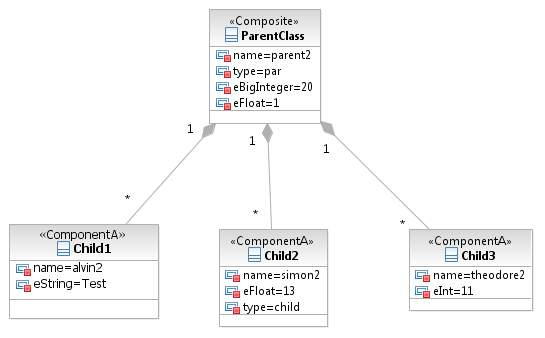
\includegraphics[scale=0.5]{CompareChildrenMatchedOrSimilarTestScreens/Testcase01model2.jpeg}

  \item[testcase\_02:]  2 Gleiche Modelle. 100\% �bereinstimmung.
    
   \begin{equation*}
   Similarity = \frac{1+1+1}{3}=1
   \end{equation*}
    
	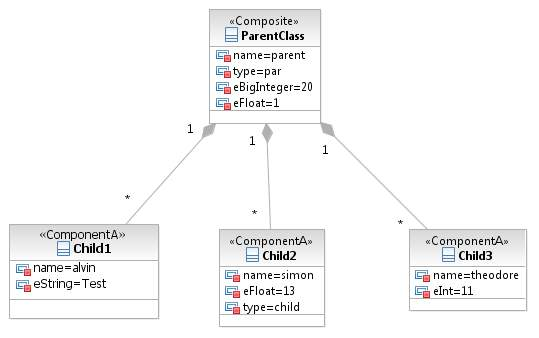
\includegraphics[scale=0.5]{CompareChildrenMatchedOrSimilarTestScreens/Testcase01model1.jpeg}
	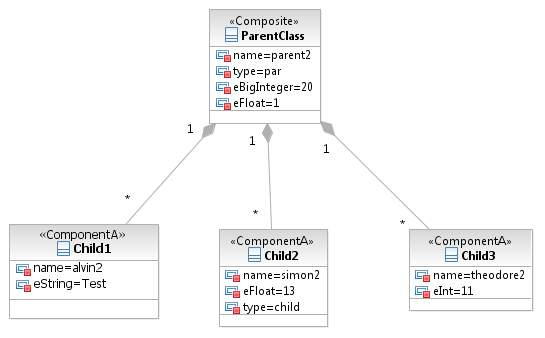
\includegraphics[scale=0.5]{CompareChildrenMatchedOrSimilarTestScreens/Testcase01model2.jpeg}

  \item[testcase\_03:] 2 Kinder sind gleich. Bei dem dritten gibt es 25\% �bereinstimmung.
    
   \begin{equation*}
   Similarity = \frac{1+1+0.25}{3}=\frac{3}{4}
   \end{equation*}
    
	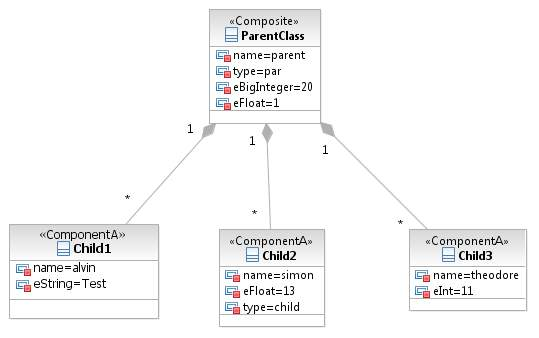
\includegraphics[scale=0.5]{CompareChildrenMatchedOrSimilarTestScreens/Testcase03model1.jpeg}
	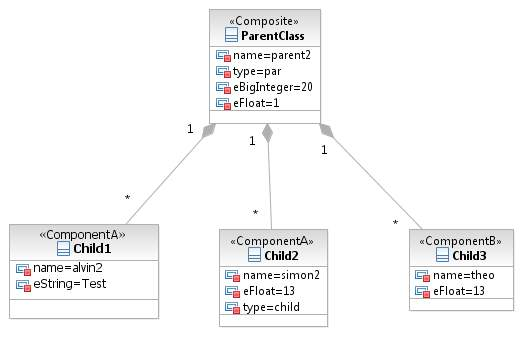
\includegraphics[scale=0.5]{CompareChildrenMatchedOrSimilarTestScreens/Testcase03model2.jpeg}

  \item[testcase\_04:]  2 Kinder sind gleich. Das dritte ist v�llig verschieden.
    
   \begin{equation*}
   Similarity = \frac{1+1+0}{3}=\frac{2}{3}
   \end{equation*}
    
	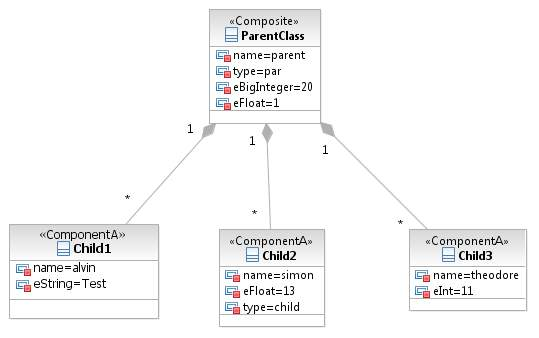
\includegraphics[scale=0.5]{CompareChildrenMatchedOrSimilarTestScreens/Testcase03model1.jpeg}
	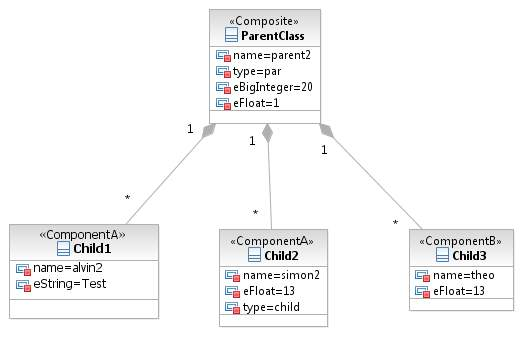
\includegraphics[scale=0.5]{CompareChildrenMatchedOrSimilarTestScreens/Testcase03model2.jpeg}

  \item[testcase\_05:]  2 Kinder sind gleich. 1 Kind fehlt (vergleich NULL).
    
   \begin{equation*}
   Similarity = \frac{1+1+0}{3}=\frac{2}{3}
   \end{equation*}
    
	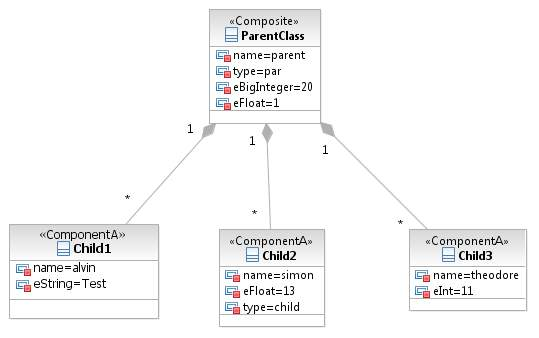
\includegraphics[scale=0.5]{CompareChildrenMatchedOrSimilarTestScreens/Testcase05model1.jpeg}
	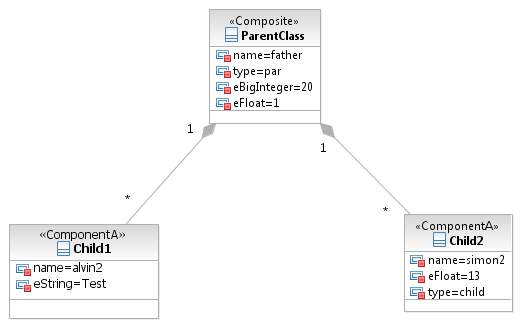
\includegraphics[scale=0.5]{CompareChildrenMatchedOrSimilarTestScreens/Testcase05model2.jpeg}

  \item[testcase\_06:]  2 Kinder sind gleich. 1 Kind fehlt (vergleich NULL).
    
   \begin{equation*}
   Similarity = \frac{1+1+0}{3}=\frac{2}{3}
   \end{equation*}
    
	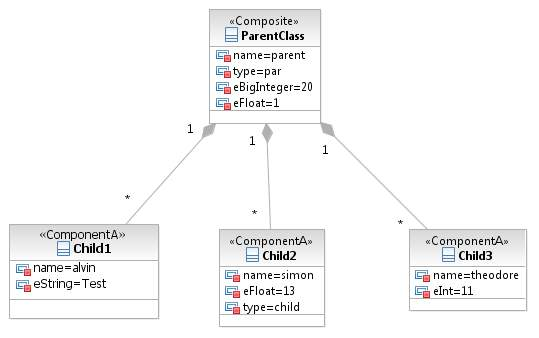
\includegraphics[scale=0.5]{CompareChildrenMatchedOrSimilarTestScreens/Testcase05model1.jpeg}
	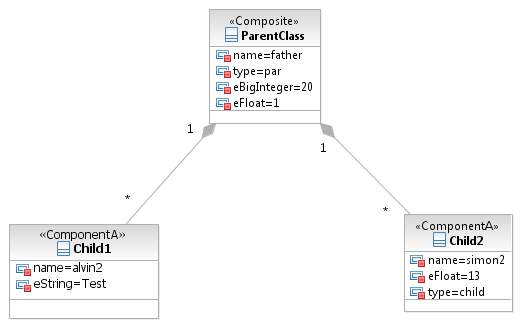
\includegraphics[scale=0.5]{CompareChildrenMatchedOrSimilarTestScreens/Testcase05model2.jpeg}

  \item[testcase\_07:] 2 Kinder sind gleich und 1 ist zu 80\% gleich.
    
   \begin{equation*}
   Similarity = \frac{1+1+0,25}{3}=\frac{3}{4}
   \end{equation*}
    
	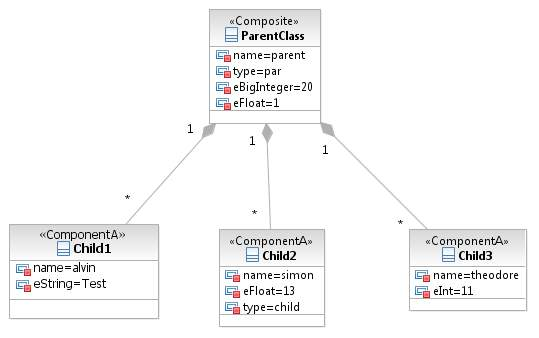
\includegraphics[scale=0.5]{CompareChildrenMatchedOrSimilarTestScreens/Testcase07model1.jpeg}
	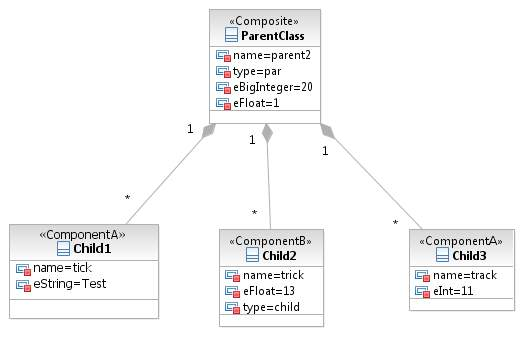
\includegraphics[scale=0.5]{CompareChildrenMatchedOrSimilarTestScreens/Testcase07model2.jpeg}

  \item[testcase\_08:] 2 Kinder sind gleich und 1 ist zu 80\% gleich.
    
   \begin{equation*}
   Similarity = \frac{1+1+0,8}{3}=\frac{14}{15}
   \end{equation*}
       
	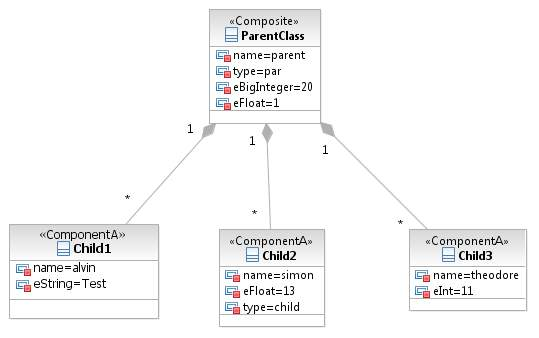
\includegraphics[scale=0.5]{CompareChildrenMatchedOrSimilarTestScreens/Testcase07model1.jpeg}
	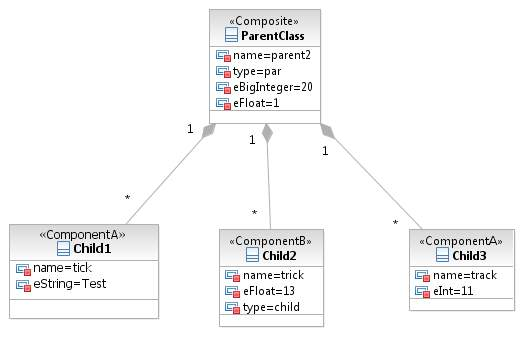
\includegraphics[scale=0.5]{CompareChildrenMatchedOrSimilarTestScreens/Testcase07model2.jpeg}

  \item[testcase\_09:] Es werden 2 voellig unterschiedliche Modelle verglichen.
    
   \begin{equation*}
   Similarity = \frac{0.1+0.2+0.1}{3}=\frac{2}{15}
   \end{equation*}
    
	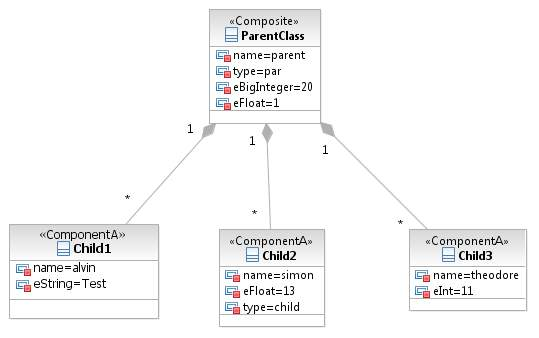
\includegraphics[scale=0.5]{CompareChildrenMatchedOrSimilarTestScreens/Testcase09model1.jpeg}
	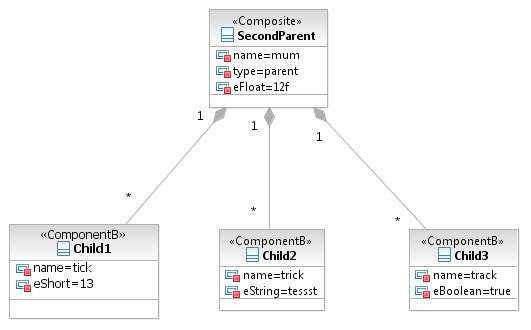
\includegraphics[scale=0.5]{CompareChildrenMatchedOrSimilarTestScreens/Testcase09model2.jpeg}

  \item[testcase\_10:] Es werden 2 voellig unterschiedliche Modelle verglichen. Alle Similarities sind 0.
    
   \begin{equation*}
   Similarity = \frac{0.4+0.6+0.5}{3}=\frac{1}{2}
   \end{equation*}
    
	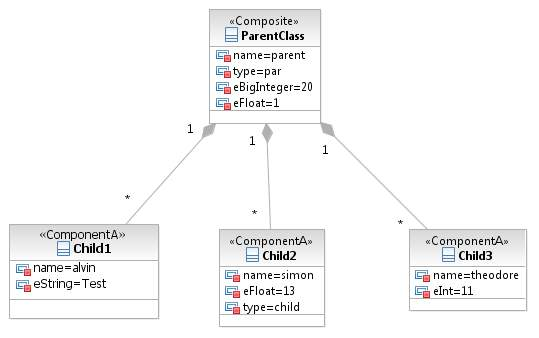
\includegraphics[scale=0.5]{CompareChildrenMatchedOrSimilarTestScreens/Testcase09model1.jpeg}
	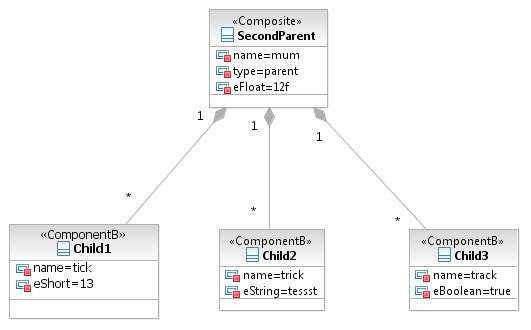
\includegraphics[scale=0.5]{CompareChildrenMatchedOrSimilarTestScreens/Testcase09model2.jpeg}
	\end{description}
	
	



\end{document}